% ch08b Quenching of local moments: the Kondo problem, part b (书页 102-114 / 分册p023-035)
%--TAIL--
式 (8.77) 对应的铁磁情形类似三重态试探波函数同样导致一个束缚态。这一不物理的结果表明，简单的变分方法不足以描述近藤模型的真实基态。所缺失的一个关键物理要素，是费米面附近 $T_{\mathrm{k}}$ 范围内所有电子对局域磁矩的集体多体淬灭。这种淬灭可以想象为在杂质周围形成一团电子云，把自旋磁矩屏蔽掉。低能标 $T_{\mathrm{k}}$ 的存在意味着，应当由一个指数般大的长度标度 $\xi_{\mathrm{k}} = \hbar v_{\mathrm{F}} / k_{\mathrm{B}} T_{\mathrm{k}}$ 来描述这个屏蔽云。对 Cu 中的 Fe 而言，$\xi_{\mathrm{k}}$ 约为 2000~\AA{}。第一个正确地纳入这些导致近藤模型基态的多体效应的尝试，是 Anderson 的“穷人标度法”，下面我们就转向这一方法。

\section{穷人标度法（Poor Man's scaling）}

多体体系在长波标度下的行为，依赖于微观自由度在所有长度标度上的相互作用。在这类体系中，短波自由度决定了长波理论的有效宏观参量。一个大家熟悉的例子是流体力学：它描述的流体，其长度和时间标度都远大于粒子的平均自由程和散射时间，其中只出现声速和粘滞系数这类有效参量；这些参量由微观物理决定。标度分析的目标，是在越来越长的波长标度上建立起一系列对体系的描述，而每一步都积分掉越来越多的较高动量标度。一经积分，较高动量标度的自由度便不再显式地出现在问题之中。自由度的稀化导致一个简化的有效模型，低能物理即可从中提取。这样，随着各种自由度被逐一积分掉，人们就为物理上重要的耦合常数建立起递推方程。

对近藤问题最简单的标度分析，是在微扰论中逐次把高能激发从中间态中消去。在每一层级上，自旋--自旋耦合常数 $J_{\mathbf{k},\mathbf{k}'}$ 都会被修改。为了看清这一方法如何运作，我们只在有效自旋--自旋耦合的二阶微扰论内做计算——“穷人标度法”之名即由此而来。虽然微扰论中的高阶项对标度也有贡献，但它们并不带来定性上的新特点 (SZ1974)。

在给出 Anderson 对各向同性近藤模型的标度分析之前，先引用其关键结果。随着温度变化，电子所探及的状态数增多，有效耦合（本节记作 $J$）服从方程
\begin{equation*}
\frac{\mathrm{d}J}{\mathrm{d}\ln(T_{\mathrm{F}}/T)} = -J^{2}N(0),
\tag{8.88}
\end{equation*}
其解即式 (8.64)。这一表达式正确地预言了近藤问题的本质物理：越来越小的能量激发（在低温下占主导）通过一个自举（bootstrapping）过程，导致交换相互作用发散，并在局域磁矩处束缚一个自旋反平行的电子 (A1978)。虽然式 (8.88) 并未消除 Kondo 早年发现的发散，但它确实阐明了交换耦合的幅值如何增大。这里可以对这一增大过程与夸克物理中色自由度的禁闭之间做一个粗略的类比 (A1978)。说这个类比粗略，是因为我们并不确切知道后者是如何实现的。

\begin{figure}[H]\centering
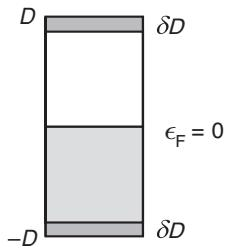
\includegraphics[width=0.42\textwidth]{figs/ch08/fig_8.7.jpg}
\caption*{图 8.7\quad 穷人标度法中要被消去的粒子态与空穴态。被移除的态的宽度为 $\delta D$。}\label{fig:auto:8.7}
\end{figure}

发展标度思想有许多途径，有简单的也有复杂的。我们将给出简单途径的一个精简版本 (H1993)。考虑一个满足 $-D < \epsilon_{\mathbf{k}} < D$ 的电子能带。如图 8.7 所示，我们的做法是分别从能带的下部和上部消去一窄层粒子态和空穴态，被消去态的宽度为 $\delta D$。基本想法是：考察进入二阶跃迁振幅的那些散射过程，确定当带宽缩减一个无穷小量 $\delta D$ 时它们如何变化。我们希望，随着带宽的缩减，能够找到一组把新的交换耦合与原有耦合联系起来的方程。

为简单起见，我们处理 $S=1/2$ 的杂质，但出于一般性的考虑，采用一个各向异性的自旋翻转哈密顿量
\begin{equation*}
H' = -\frac{1}{2\hbar V} \sum_{\mathbf{k}',\mathbf{k}'',\sigma} \Big[ J_{z} S_{d}^{z} \big( a_{\mathbf{k}'\uparrow}^{\dagger} a_{\mathbf{k}''\uparrow} - a_{\mathbf{k}'\downarrow}^{\dagger} a_{\mathbf{k}''\downarrow} \big) + J_{+} S_{d}^{+} a_{\mathbf{k}'\downarrow}^{\dagger} a_{\mathbf{k}''\uparrow} + J_{-} S_{d}^{-} a_{\mathbf{k}'\uparrow}^{\dagger} a_{\mathbf{k}''\downarrow} \Big],
\end{equation*}
其中自旋翻转部分（$J_{\pm}$）与纵向部分（$J_{z}$）具有不同的相互作用强度。我们的目标是化简二阶微扰项，证明它们导致 $J_{z}$ 与 $J_{\pm}$ 裸值的重正化。首先考虑图 8.8 所示的两个自旋翻转过程。由于双自旋翻转过程不改变杂质自旋，我们预期双自旋翻转项将导致纵向耦合 $J_{z}$ 的重正化。对 $J_{z}$ 修正的精确形式，可以对每一幅双自旋翻转图实施标度分析而得到。考虑第一幅图：
\begin{equation*}
J_{+}J_{-} \sum_{\mathbf{q}} \frac{S_{d}^{-}}{2\hbar V} a_{\mathbf{k}'\uparrow}^{\dagger} a_{\mathbf{q}\downarrow} \big( E - \widehat{H}_{0} \big)^{-1} \sum_{\mathbf{q}'} \frac{S_{d}^{+}}{2\hbar V} a_{\mathbf{q}'\downarrow}^{\dagger} a_{\mathbf{k}\uparrow}.
\tag{8.89}
\end{equation*}

\begin{figure}[H]\centering
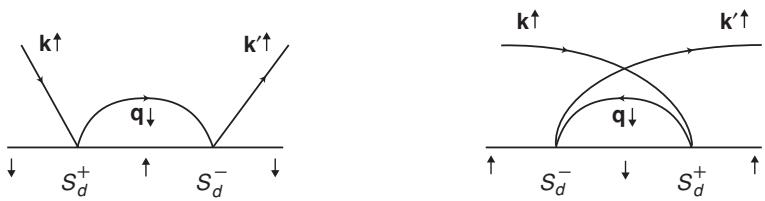
\includegraphics[width=0.72\textwidth]{figs/ch08/fig_8.8.jpg}
\caption*{图 8.8\quad 中间态包含粒子或空穴的二阶双自旋翻转图。实直线表示杂质自旋，曲线表示电子。}\label{fig:auto:8.8}
\end{figure}

为实施标度程序，我们把对 $\mathbf{q}'$ 的求和限制在距带顶 $\delta D$ 以内的状态，这些态由 $a_{\mathbf{q}'\downarrow}^{\dagger}$ 产生。由于带边态本来未被占据，必须取 $a_{\mathbf{q}} a_{\mathbf{q}'}^{\dagger} = \delta_{\mathbf{q},\mathbf{q}'}$。

在化简式 (8.89) 时，不能随意把最右边的产生和湮灭算符移过算符 $1/(E-\widehat{H}_{0})$，因为它们与 $\widehat{H}_{0}$ 不对易。对任一满足 $[\widehat{H}_{0}, \widehat{A}] = b\widehat{A}$ 的算符 $\widehat{A}$（其中 $b$ 是一个 c 数（c-number）），有 $\widehat{H}_{0}^{\,n}\widehat{A} = \widehat{A}(b + \widehat{H}_{0})^{n}$。于是
\begin{align*}
\frac{1}{E-\widehat{H}_{0}}\,\widehat{A} &= \frac{\widehat{A}}{E} \sum_{n=0}^{\infty} \frac{(\widehat{H}_{0}+b)^{n}}{E^{n}} \tag{8.90}\\
&= \widehat{A}\,\frac{1}{E-b-\widehat{H}_{0}}. \tag{8.91}
\end{align*}
利用 $[\widehat{H}_{0}, a_{\mathbf{q}'\downarrow}^{\dagger} a_{\mathbf{k}\uparrow}] = a_{\mathbf{q}'\downarrow}^{\dagger} a_{\mathbf{k}\uparrow} (\epsilon_{\mathbf{q}'} - \epsilon_{\mathbf{k}})$ 这一事实，我们把式 (8.89) 中的矩阵元化简为
\begin{equation*}
J_{+}J_{-} N(0)|\delta D| \frac{S_{d}^{-}S_{d}^{+}}{4V\hbar^{2}} a_{\mathbf{k}'\uparrow}^{\dagger} a_{\mathbf{k}\uparrow} \big( E - \epsilon_{\mathbf{q}} + \epsilon_{\mathbf{k}} - \widehat{H}_{0} \big)^{-1}.
\tag{8.92}
\end{equation*}
由于出现了 $a_{\mathbf{k}'\uparrow}^{\dagger} a_{\mathbf{k}\uparrow}$ 型的依赖，可以清楚地看到，双自旋翻转项改变了裸横向交换相互作用的取值。为提取精确的系数，我们利用 $S_{d}^{-}S_{d}^{+} = \hbar^{2}/2 - \hbar S_{d}^{z}$ 并取 $\epsilon_{\mathbf{q}} = D$。此外，若从带底量度 $E$，则可以忽略式 (8.92) 分母中 $\widehat{H}_{0}$ 的依赖。矩阵元化简为
\begin{equation*}
J_{+}J_{-} N(0) \frac{|\delta D|}{4\hbar V} \left( \frac{\hbar}{2} - S_{d}^{z} \right) a_{\mathbf{k}'\uparrow}^{\dagger} a_{\mathbf{k}\uparrow} \big( E - D + \epsilon_{\mathbf{k}} \big)^{-1}.
\tag{8.93}
\end{equation*}
现在可以用同样的方式计算图 8.8 中的第二幅图。这里中间态是粒子态，因此取 $\epsilon_{\mathbf{q}} = -D$，得到
\begin{equation*}
J_{+}J_{-} N(0) \frac{|\delta D|}{4\hbar V} \left( \frac{\hbar}{2} + S_{d}^{z} \right) a_{\mathbf{k}\uparrow} a_{\mathbf{k}'\uparrow}^{\dagger} \big( E - D - \epsilon_{\mathbf{k}'} \big)^{-1}.
\tag{8.94}
\end{equation*}
在推导此结果时，我们利用了关系式 $S_{d}^{+}S_{d}^{-} = \hbar^{2}/2 + \hbar S_{d}^{z}$。

其余涉及双自旋翻转的标度方程，可以通过计入来自 $\mathbf{k}\downarrow$ 与 $\mathbf{k}'\downarrow$ 的贡献得到。自旋向下状态之间的散射会产生正比于 $a_{\mathbf{k}\downarrow} a_{\mathbf{k}'\downarrow}^{\dagger}$ 的矩阵元，这一项将对 $S_{z}$ 算符的 $m_{s} = -1$ 自旋分量有贡献。

\begin{figure}[H]\centering
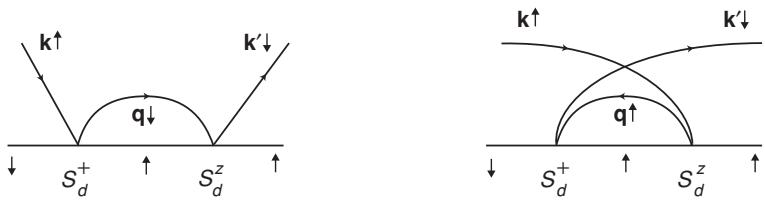
\includegraphics[width=0.72\textwidth]{figs/ch08/fig_8.9.jpg}
\caption*{图 8.9\quad 中间态包含粒子或空穴的二阶单自旋翻转图。实直线表示杂质自旋，曲线表示电子。}\label{fig:auto:8.9}
\end{figure}

现在定义新的纵向相互作用 $J_{z} \to J_{z} + \delta J_{z}$。注意到式 (8.89) 中裸相互作用的系数为 $1/2\hbar V$，我们发现式 (8.93) 与式 (8.94) 再结合自旋向下的方程，给出
\begin{equation*}
\delta J_{z} = \frac{1}{2} J_{+}J_{-} N(0)|\delta D| \left[ \frac{1}{E-D+\epsilon_{\mathbf{k}}} + \frac{1}{E-D-\epsilon_{\mathbf{k}'}} \right]
\tag{8.95}
\end{equation*}
作为对 $J_{z}$ 的修正。$J_{z}$ 的重正化依赖于能量。现在考虑能量远低于 $D$ 的激发，并在费米能级 $\epsilon_{\mathrm{F}} = 0$ 处取 $\epsilon_{\mathbf{k}}$ 与 $\epsilon_{\mathbf{k}'}$ 的值，$J_{z}$ 的标度方程便简化为
\begin{equation*}
\frac{\mathrm{d}J_{z}}{\mathrm{d}\ln D} = N(0)J_{\pm}^{2},
\tag{8.96}
\end{equation*}
其中我们已取 $\delta D$ 为负，并令 $J_{+} = J_{-} = J_{\pm}$。

现在考虑图 8.9 所示的单自旋翻转项。第一幅图的形式为
\begin{equation*}
- J_{+}J_{z} \sum_{\mathbf{q}} \frac{S_{d}^{z}}{2\hbar V} a_{\mathbf{k}'\downarrow}^{\dagger} a_{\mathbf{q}\downarrow} \big( E - \widehat{H}_{0} \big)^{-1} \sum_{\mathbf{q}'} \frac{S_{d}^{+}}{2\hbar V} a_{\mathbf{q}'\downarrow}^{\dagger} a_{\mathbf{k}'\uparrow}.
\tag{8.97}
\end{equation*}
该式前端的负号来源于 $S_{d}^{z}$ 的自旋向下分量所带的负号。用与双自旋翻转情形相同的技术，我们把该矩阵元化为
\begin{equation*}
\frac{- J_{+}J_{z} N(0)|\delta D| S_{d}^{+} a_{\mathbf{k}'\downarrow}^{\dagger} a_{\mathbf{k}\uparrow}}{8\hbar V \big( E - D + \epsilon_{\mathbf{k}} \big)},
\tag{8.98}
\end{equation*}
其中用到了 $S_{d}^{z}S_{d}^{+} = \hbar S_{d}^{+}/2$ 这一事实。因此，自旋翻转相互作用的重正化涉及 $J$ 的纵向分量。类似地，图 8.9 中另一幅图的取值为
\begin{equation*}
\frac{J_{+}J_{z} N(0)|\delta D| S_{d}^{+} a_{\mathbf{k}\uparrow} a_{\mathbf{k}'\downarrow}^{\dagger}}{8\hbar V \big( E - D - \epsilon_{\mathbf{k}'} \big)}.
\tag{8.99}
\end{equation*}
交换 $S_{d}^{z}$ 与 $S_{d}^{+}$ 的先后次序，可以得到这一形式的更多贡献，此时应使用恒等式 $S_{d}^{+}S_{d}^{z} = -\hbar S_{d}^{+}/2$。这里的贡献与式 (8.98) 和式 (8.99) 中的完全相同。

类似地，我们把单自旋翻转的结果与自旋向下电子散射的结果结合起来。定义新的横向相互作用 $J_{\pm}/2 \to (J_{\pm} + \delta J_{\pm})/2$，并利用式 (8.98) 与式 (8.99) 的结果，便得到交换相互作用横向分量的标度方程
\begin{equation*}
\delta J_{\pm} = \frac{1}{2} J_{\pm}J_{z} N(0)|\delta D| \left[ \frac{1}{E-D+\epsilon_{\mathbf{k}}} + \frac{1}{E-D-\epsilon_{\mathbf{k}'}} \right]
\tag{8.100}
\end{equation*}
这里同样地，横向耦合常数的标度依赖于能量。与纵向情形一样，我们考虑能量远低于 $D$ 的激发，并在费米能级 $\epsilon_{\mathrm{F}} = 0$ 处取 $\epsilon_{\mathbf{k}}$ 与 $\epsilon_{\mathbf{k}'}$ 的值，标度方程便简化为
\begin{equation*}
\frac{\mathrm{d}J_{\pm}}{\mathrm{d}\ln D} = N(0)J_{z}J_{\pm}.
\tag{8.101}
\end{equation*}

取式 (8.96) 与式 (8.101) 之比并积分，可以看到解是由
\begin{equation*}
J_{z}^{2} - J_{\pm}^{2} = \kappa,
\tag{8.102}
\end{equation*}
确定的一族双曲线，其中 $\kappa$ 为常数。为提取这些标度方程的物理结论，把式 (8.102) 代入 $J_{\pm}$ 的标度方程是有益的。对铁磁与反铁磁两种情形，我们发现
\begin{equation*}
\frac{\mathrm{d}J_{\pm}}{\mathrm{d}|\ln D|} =
\begin{cases}
-N(0)J_{\pm}\sqrt{\kappa + J_{\pm}^{2}}, & \quad J_{z} > 0, \quad \text{铁磁},\\
\phantom{-}N(0)J_{\pm}\sqrt{\kappa + J_{\pm}^{2}}, & \quad J_{z} < 0, \quad \text{反铁磁}.
\end{cases}
\tag{8.103}
\end{equation*}

标度分析的物理结论现在清楚了。由于式 (8.103) 的右端在 $J_{z} > 0$ 时为负，标度方程规定在此情形下 $J_{\pm} \to 0$。结果，在铁磁情形，横向交换耦合随带宽的缩减变得越来越弱。然而，在反铁磁情形，式 (8.103) 的右端为正，标度方程规定 $|J_{\pm}| \to \infty$。这就是发生近藤效应的强耦合区域。交换耦合的幅值随带宽的减小而增大。正是交换相互作用在带宽减小时被自举到更大的数值，导致了近藤杂质处单态的形成。

图 8.10 所示的流图使标度分析一目了然。双曲线是各向异性耦合（$|J_{+}| > |J_{z}|$）的结果，直线则是各向同性耦合极限下解坍缩为 $|J_{+}|^{2} = J_{z}^{2}$ 的情形。箭头指向 $D$ 减小的方向。$J_{z}$ 为正（铁磁耦合）的曲线表明，随着 $D$ 趋于零，$J_{z}$ 与 $|J_{+}|$ 流向零；而 $J_{z}$ 为负（反铁磁耦合）的曲线则表明，随着 $D$ 趋于零，两个耦合都发散。各向同性极限与各向异性极限展现出相同的物理。

\begin{figure}[H]\centering
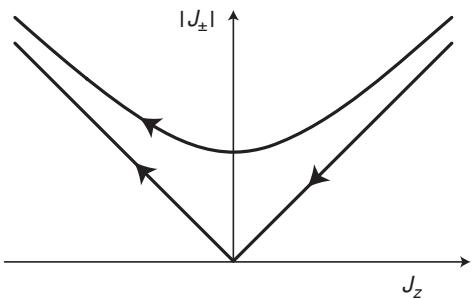
\includegraphics[width=0.5\textwidth]{figs/ch08/fig_8.10.jpg}
\caption*{图 8.10\quad 用 Anderson 的二阶微扰论论证得到的近藤模型标度轨迹。双曲线对应各向异性耦合，直线对应各向同性耦合。$J_{z} > 0$ 的区域对应铁磁耦合，$J_{z} < 0$ 的区域对应反铁磁耦合。}\label{fig:auto:8.10}
\end{figure}

在各向同性极限下，$J_{\pm}(D) = J_{z}(D) = J(D)$，标度方程约化为单一方程
\begin{equation*}
\frac{\mathrm{d}J}{\mathrm{d}\ln D} = J^{2}N(0),
\tag{8.104}
\end{equation*}
其解为
\begin{equation*}
J(D) = \frac{J(D_{0})}{1 - J(D_{0})N(0)\ln(D/D_{0})},
\tag{8.105}
\end{equation*}
其中 $D_{0}$ 是初始带宽。物理上，我们感兴趣的情形是：有效带宽处于有限温度下电子所能探及的状态范围，即费米面附近宽度为 $k_{\mathrm{B}}T$ 的区间。于是在对数精度下可以取 $D/D_{0} = k_{\mathrm{B}}T/\epsilon_{\mathrm{F}} = T/T_{\mathrm{F}}$。作了这一认定后，式 (8.105) 与式 (8.64) 完全等价。

下面从标度方程中提取近藤温度。这样做时，重要的是记住近藤温度是一个物理量，因而不应依赖于我们在模型描述中选取的带宽 $D$，也就是说，$T_{\mathrm{k}}$ 应当是标度不变的，
\begin{equation*}
D\frac{\partial T_{\mathrm{k}}}{\partial D} = 0.
\tag{8.106}
\end{equation*}
这样一来，所有物理量（如电阻率和磁化率）都将依赖于比值 $T/T_{\mathrm{k}}$（对 $T/T_{\mathrm{F}}$ 的依赖则奇异性较弱），而不依赖于 $D$。

如果我们在各向同性情形下定义无量纲耦合常数 $g = N(0)J$，标度方程便成为
\begin{equation*}
\frac{\mathrm{d}g}{\mathrm{d}\ln D} \equiv \beta(g) = g^{2}.
\tag{8.107}
\end{equation*}
耦合常数的对数导数通常称为 $\beta$ 函数，得名于盖尔曼（Gell-Mann）和洛（Low）(GL1954)；在第 13 章讨论局域化时我们还会遇到这个概念。从量纲上看，近藤温度必须具有 $k_{\mathrm{B}}T_{\mathrm{k}} = Dy(g)$ 的形式，其中 $D$ 确定能标。为确定 $y$，把 $T_{\mathrm{k}}$ 的这一形式代入标度不变条件，即式 (8.106)，得到线性微分方程
\begin{equation*}
y(g) + \frac{\partial y}{\partial g}\frac{\partial g}{\partial \ln D} = 0.
\tag{8.108}
\end{equation*}
其解很简单：
\begin{equation*}
y(g) \sim \mathrm{e}^{1/g}.
\tag{8.109}
\end{equation*}
因此，近藤温度由 $k_{\mathrm{B}}T_{\mathrm{k}} = D\exp(1/(N(0)J))$ 给出，与我们先前看到的式 (8.86) 的结构一致。近藤温度与带宽无关，而前面却又显含因子 $D$，这看似矛盾，其实不然。对 $D$ 的补偿性依赖藏在耦合常数 $g$ 之中，使得式 (8.106) 得以满足。

近藤问题的完整标度结构，由威尔逊（Wilson）在对该问题的关键性重正化群分析 (W1975) 中确定。威尔逊证明，随着能标趋于零，本征态的分布变得大致等价于 $J \to -\infty$ 的体系的分布。因此，初始具有小交换相互作用的体系，随着能标的降低，平滑地交叉过渡（crossover）到交换相互作用向负方向发散的体系。正是相互作用的发散导致了近藤问题中向单态基态的交叉过渡。不过，在威尔逊重正化群方法中，发散发生在 $T = 0$，而不是在有限的 $T_{\mathrm{k}}$ 处；这里 $T_{\mathrm{k}}$ 处的发散，是微扰论中领头对数（leading logarithm）求和造成的假象。

至此，关于近藤问题的故事大体讲完了。不过，更晚近的理论工作还包括：Nozières (N1974) 关于 $T_{\mathrm{k}}$ 以下费米液体图像的工作、Anderson 模型与近藤模型的精确贝特拟设（Bethe ansatz）解 (TW1983; AFL1983)，以及共形场论方法 (AL1991; AZ1996)。计入电子关联 (LT1992) 会使近藤温度随交换耦合按代数（幂律）方式而非指数方式标度，这与这里讨论的不同；其幂指数正比于导带电子之间相互作用的强度。此外，理论预言即使对铁磁相互作用，近藤单态也可以稳定存在 (FN1994)，这一结果是在卢廷格液体的框架内建立的，我们将在第 10 章讨论。

\section*{小结}
\addcontentsline{toc}{section}{小结}

低温下金属中局域磁矩的淬灭，正是近藤问题背后的物理。这一效应来源于钉扎在费米能级上的多体共振。本章我们着重于从相当简单的考虑出发提取这一图像。近藤温度是一个标度不变量，由 $T_{\mathrm{k}} = D\exp(1/g)$ 给出，其中 $g = N(0)J$ 是有效裸近藤交换相互作用。从微扰的角度看，近藤温度可以认定为这样的能标：在此能标处，微扰论中的二阶项变得与 $J$ 的线性项同量级——这是微扰论正在失效、高阶项同样重要的标志。费米能级处的共振是真正的多粒子效应：微扰论中的 $n$ 阶项包含 $n$ 个电子与局域磁矩的相互作用。正是对所有这些项的求和产生了共振。

\section*{本章附录：Schrieffer--Wolff 变换}
\addcontentsline{toc}{section}{本章附录：Schrieffer--Wolff 变换}

在本附录中，我们从 Anderson 哈密顿量出发，完整地推导近藤哈密顿量中的交换相互作用。由于 Anderson 哈密顿量既包含空的也包含双占据的杂质态，一个生成近藤哈密顿量的变换，等价于把 Anderson 哈密顿量在单占据杂质态的子空间内对角化。这一对角化由 Schrieffer--Wolff 变换 (SW1966) 完成。

我们先把 Anderson 哈密顿量分解为零阶部分
\begin{equation*}
H_{0} = \sum_{\mathbf{k},\sigma} \epsilon_{\mathbf{k}} n_{\mathbf{k}\sigma} + \epsilon_{d} \sum_{\sigma} n_{d\sigma} + U n_{d\uparrow} n_{d\downarrow}
\tag{8.110}
\end{equation*}
和微扰部分
\begin{equation*}
H_{1} = \sum_{\mathbf{k}\sigma} V_{\mathbf{k}d} \big( a_{\mathbf{k}\sigma}^{\dagger} a_{d\sigma} + a_{d\sigma}^{\dagger} a_{\mathbf{k}\sigma} \big).
\tag{8.111}
\end{equation*}
在本推导中，取 $V_{\mathbf{k}d}$ 为实数。

为推进推导，我们对原哈密顿量施行一个正则变换（或相似变换）$S$：
\begin{equation*}
\begin{aligned}
\widetilde{H} &= \mathrm{e}^{S} H \mathrm{e}^{-S} \\
&= H + [S, H] + \frac{1}{2}[S, [S, H]] + \cdots.
\end{aligned}
\end{equation*}
注意，由于 $\mathrm{e}^{S}$ 是幺正的，$S$ 必须是反厄米的。如果选取 $S$ 使之消去对微扰 $H_{1}$ 的线性依赖，即
\begin{equation*}
H_{1} + [S, H_{0}] = 0
\tag{8.112}
\end{equation*}
那么精确到最低阶的新哈密顿量为
\begin{equation*}
\widetilde{H} = H_{0} + \frac{1}{2}[S, H_{1}],
\tag{8.113}
\end{equation*}
从而把电荷涨落纳入到 $V_{\mathbf{k}d}$ 的二阶。一旦辨识出小量，相似变换方法就是进行微扰分析的一种一般方法。

$S$ 的显式形式可以这样构造：注意到由于 $[S, H_{0}] = -H_{1}$，算符 $S$ 必须含有正比于 $a_{\mathbf{k}\sigma}^{\dagger} a_{d\sigma}$ 的项；此外，它与 $U n_{d\uparrow} n_{d\downarrow}$ 的对易子给出正比于 $n_{d-\sigma} a_{\mathbf{k}\sigma}^{\dagger} a_{d\sigma}$ 的项。这提示我们尝试如下形式的变换
\begin{equation*}
S = \sum_{\mathbf{k},\sigma} \big( A_{\mathbf{k}} + B_{\mathbf{k}} n_{d-\sigma} \big) a_{\mathbf{k}\sigma}^{\dagger} a_{d\sigma} - \mathrm{h.c.},
\tag{8.114}
\end{equation*}
其中 $A_{\mathbf{k}}$ 与 $B_{\mathbf{k}}$ 是有待由式 (8.112) 确定的 c 数。

利用如下对易关系：
\begin{equation*}
\begin{aligned}
& \big[ n_{d\sigma}, a_{d\sigma'} \big] = -\delta_{\sigma\sigma'} a_{d\sigma}, \\
& \big[ n_{d\sigma}, n_{d\sigma'} \big] = 0, \\
& \big[ n_{d\sigma} n_{d-\sigma}, a_{d\sigma'} \big] = -\delta_{\sigma\sigma'} n_{d-\sigma} a_{d\sigma} - \delta_{-\sigma\sigma'} n_{d\sigma} a_{d\sigma'},
\end{aligned}
\tag{8.115}
\end{equation*}
再加上关系式 $[A, B^{\dagger}] = -[A, B]^{\dagger}$（当 $A = A^{\dagger}$ 时成立），我们直接计算 $H_{0}$ 与 $S$ 的对易子，得到
\begin{align*}
[H_{0}, S] = {} & \sum_{\mathbf{k},\sigma} \epsilon_{\mathbf{k}} \big( A_{\mathbf{k}} + B_{\mathbf{k}} n_{d-\sigma} \big) a_{\mathbf{k}\sigma}^{\dagger} a_{d\sigma} + \mathrm{h.c.} + \sum_{\mathbf{k},\sigma} \epsilon_{d} \big( -A_{\mathbf{k}} - B_{\mathbf{k}} n_{d-\sigma} \big) a_{\mathbf{k}\sigma}^{\dagger} a_{d\sigma} + \mathrm{h.c.} \\
& + U \sum_{\mathbf{k},\sigma} \big( -A_{\mathbf{k}} n_{d-\sigma} - B_{\mathbf{k}} n_{d-\sigma} \big) a_{\mathbf{k}\sigma}^{\dagger} a_{d\sigma} + \mathrm{h.c.} \\
= {} & \sum_{\mathbf{k},\sigma} \big[ (\epsilon_{\mathbf{k}} - \epsilon_{d}) A_{\mathbf{k}} + (\epsilon_{\mathbf{k}} - \epsilon_{d} - U) n_{d-\sigma} B_{\mathbf{k}} - A_{\mathbf{k}} U n_{d-\sigma} \big] a_{\mathbf{k}\sigma}^{\dagger} a_{d\sigma} + \mathrm{h.c.}, \tag{8.116}
\end{align*}
其中 h.c. 表示厄米共轭。为满足式 (8.112)，我们要求 $(\epsilon_{\mathbf{k}} - \epsilon_{d}) A_{\mathbf{k}} = V_{\mathbf{k}d}$ 以及 $(\epsilon_{\mathbf{k}} - \epsilon_{d} - U) B_{\mathbf{k}} - A_{\mathbf{k}} U = 0$，于是
\begin{equation*}
A_{\mathbf{k}} = \frac{V_{\mathbf{k}d}}{\epsilon_{\mathbf{k}} - \epsilon_{d}}
\end{equation*}
且
\begin{equation*}
B_{\mathbf{k}} = V_{\mathbf{k}d} \left[ \frac{1}{\epsilon_{\mathbf{k}} - (\epsilon_{d} + U)} - \frac{1}{\epsilon_{\mathbf{k}} - \epsilon_{d}} \right].
\end{equation*}
式 (8.114) 连同常数 $A_{\mathbf{k}}$、$B_{\mathbf{k}}$ 的这组定义，就完全确定了 Schrieffer--Wolff 变换。

为求新哈密顿量，需要计算对易子 $[S, H_{1}]$：
\begin{align*}
[S, H_{1}] = \sum_{\mathbf{k},\sigma,\mathbf{k}',\sigma'} \big\{ {} & A_{\mathbf{k}} V_{\mathbf{k}'d} \big[ \rho_{\mathbf{k}d\sigma}, \big( \rho_{\mathbf{k}'d\sigma'} + \rho_{\mathbf{k}'d\sigma'}^{\dagger} \big) \big] - B_{\mathbf{k}}^{*} V_{\mathbf{k}'d} \big[ n_{d-\sigma} \rho_{\mathbf{k}d\sigma}^{\dagger}, \big( \rho_{\mathbf{k}'d\sigma'} + \rho_{\mathbf{k}'d\sigma'}^{\dagger} \big) \big] \\
& + B_{\mathbf{k}} V_{\mathbf{k}'d} \big[ n_{d-\sigma} \rho_{\mathbf{k}d\sigma}, \big( \rho_{\mathbf{k}'d\sigma'} + \rho_{\mathbf{k}'d\sigma'}^{\dagger} \big) \big] - A_{\mathbf{k}}^{*} V_{\mathbf{k}'d} \big[ \rho_{\mathbf{k}d\sigma}^{\dagger}, \big( \rho_{\mathbf{k}'d\sigma'} + \rho_{\mathbf{k}'\sigma'}^{\dagger} \big) \big] \big\}, \tag{8.117}
\end{align*}
这里通过定义 $\rho_{\mathbf{k}d\sigma} = a_{\mathbf{k}\sigma}^{\dagger} a_{d\sigma}$ 简化了记号。在这一步，下列对易关系很有用：
\begin{equation*}
\begin{aligned}
& \big[ \rho_{\mathbf{k}d\sigma}, \rho_{\mathbf{k}'d\sigma'} \big] = 0, \\
& \big[ \rho_{\mathbf{k}d\sigma}, \rho_{\mathbf{k}'d\sigma'}^{\dagger} \big] = \delta_{\sigma\sigma'} \big[ -\delta_{\mathbf{k}\mathbf{k}'} n_{d\sigma} + a_{\mathbf{k}\sigma}^{\dagger} a_{\mathbf{k}'\sigma} \big], \\
& \big[ n_{d-\sigma} \rho_{\mathbf{k}d\sigma}, \rho_{\mathbf{k}'d\sigma'} \big] = -\delta_{\sigma'-\sigma} \rho_{\mathbf{k}d\sigma} \rho_{\mathbf{k}'d-\sigma}, \\
& \big[ n_{d-\sigma} \rho_{\mathbf{k}d\sigma}, \rho_{\mathbf{k}'d\sigma'}^{\dagger} \big] = \delta_{-\sigma\sigma'} \rho_{\mathbf{k}d\sigma} \rho_{\mathbf{k}'d-\sigma}^{\dagger} + \delta_{\sigma\sigma'} \big( a_{\mathbf{k}\sigma}^{\dagger} a_{\mathbf{k}'\sigma} n_{d-\sigma} - \delta_{\mathbf{k}\mathbf{k}'} n_{d-\sigma} n_{d\sigma} \big).
\end{aligned}
\end{equation*}
把这些关系代入式 (8.117)，得到
\begin{align*}
[S, H_{1}] = {} & -\sum_{\mathbf{k},\sigma} \big( A_{\mathbf{k}} V_{\mathbf{k}d} + B_{\mathbf{k}} V_{\mathbf{k}d} n_{d-\sigma} \big) n_{d\sigma} + \mathrm{h.c.} + \sum_{\mathbf{k},\mathbf{k}',\sigma} A_{\mathbf{k}} V_{\mathbf{k}'d} a_{\mathbf{k}\sigma}^{\dagger} a_{\mathbf{k}'\sigma} + \mathrm{h.c.} \\
& -\sum_{\mathbf{k},\mathbf{k}',\sigma} B_{\mathbf{k}} V_{\mathbf{k}'d} \rho_{\mathbf{k}\sigma} \rho_{\mathbf{k}'-\sigma} + \mathrm{h.c.} + \sum_{\mathbf{k},\mathbf{k}',\sigma} B_{\mathbf{k}} V_{\mathbf{k}'d} \big[ a_{\mathbf{k}\sigma}^{\dagger} a_{\mathbf{k}'\sigma} n_{d-\sigma} + \rho_{\mathbf{k}\sigma} \rho_{\mathbf{k}'-\sigma}^{\dagger} \big] + \mathrm{h.c.} \tag{8.118}
\end{align*}

把最后一项中的算符写成
\begin{equation*}
\begin{aligned}
& \big[ a_{\mathbf{k}\sigma}^{\dagger} a_{\mathbf{k}'\sigma} n_{d-\sigma} + \rho_{\mathbf{k}d\sigma} \rho_{\mathbf{k}'d-\sigma}^{\dagger} \big] = \frac{1}{2} \big( n_{d\sigma} + n_{d-\sigma} \big) a_{\mathbf{k}\sigma}^{\dagger} a_{\mathbf{k}'\sigma} \\
& \qquad - \frac{1}{2} \big[ \big( n_{d\sigma} - n_{d-\sigma} \big) a_{\mathbf{k}\sigma}^{\dagger} a_{\mathbf{k}'\sigma} - 2 \rho_{\mathbf{k}d\sigma} \rho_{\mathbf{k}'d-\sigma}^{\dagger} \big].
\end{aligned}
\tag{8.119}
\end{equation*}
这一项的第二部分给出近藤交换相互作用。为看出这一点，注意到乘积
\begin{align*}
\frac{4}{\hbar^{2}} \big( \Psi_{\mathbf{k}'}^{\dagger} \mathbf{S} \Psi_{\mathbf{k}} \big) \cdot \big( \Psi_{d}^{\dagger} \mathbf{S} \Psi_{d} \big) ={} & \big( \Psi_{\mathbf{k}'}^{\dagger} \sigma_{z} \Psi_{\mathbf{k}} \big) \cdot \big( \Psi_{d}^{\dagger} \sigma_{z} \Psi_{d} \big) + 2 \big( \Psi_{\mathbf{k}'}^{\dagger} \sigma^{+} \Psi_{\mathbf{k}} \big) \big( \Psi_{d}^{\dagger} \sigma^{-} \Psi_{d} \big) \\
& + 2 \big( \Psi_{\mathbf{k}'}^{\dagger} \sigma^{-} \Psi_{\mathbf{k}} \big) \big( \Psi_{d}^{\dagger} \sigma^{+} \Psi_{d} \big) \\
={}& \sum_{\sigma} \big[ a_{\mathbf{k}'\sigma}^{\dagger} a_{\mathbf{k}\sigma} \big( n_{d\sigma} - n_{d-\sigma} \big) - 2 \rho_{\mathbf{k}'d\sigma} \rho_{\mathbf{k}d-\sigma}^{\dagger} \big] \tag{8.120}
\end{align*}
恰好具有式 (8.119) 最后一项的形式。对 $\widetilde{H}$ 的相应贡献是
\begin{equation*}
H_{\mathrm{exch}} = -\frac{1}{\hbar^{2}} \sum_{\mathbf{k},\mathbf{k}'} J_{\mathbf{k}\mathbf{k}'} \big( \Psi_{\mathbf{k}'}^{\dagger} \mathbf{S} \Psi_{\mathbf{k}} \big) \cdot \big( \Psi_{d}^{\dagger} \mathbf{S} \Psi_{d} \big),
\tag{8.121}
\end{equation*}
其中
\begin{equation*}
\begin{aligned}
J_{\mathbf{k}\mathbf{k}'} &= \big( B_{\mathbf{k}'} V_{\mathbf{k}d} + B_{\mathbf{k}}^{*} V_{\mathbf{k}'d} \big) \\
&= V_{\mathbf{k}'d} V_{\mathbf{k}d} \left[ \frac{1}{\epsilon_{\mathbf{k}'} - (\epsilon_{d} + U)} + \frac{1}{\epsilon_{\mathbf{k}} - (\epsilon_{d} + U)} - \frac{1}{\epsilon_{\mathbf{k}} - \epsilon_{d}} - \frac{1}{\epsilon_{\mathbf{k}'} - \epsilon_{d}} \right].
\end{aligned}
\tag{8.122}
\end{equation*}

这一项来源于式 (8.119) 的最后一项，它就是近藤相互作用。注意，这个结果就是由二阶微扰论导出的式 (8.10) 的形式，只是对 $\mathbf{k}$ 与 $\mathbf{k}'$ 对称化了。我们在这里看到了相似变换方法的一个特别优点：即使初末态能量不同，它也能正确地给出相互作用矩阵元。相比之下，只有当初末态具有相同能量时，我们才能把二阶散射振幅与相互作用矩阵元等同起来，此时式 (8.10) 与式 (8.122) 一致。在费米能级附近，$k, k' \sim k_{\mathrm{F}}$，自旋交换振幅约化为
\begin{equation*}
J_{k_{\mathrm{F}} k_{\mathrm{F}}} \equiv J_{0} = -2 V_{\mathbf{k}d}^{2} \frac{U}{|\epsilon_{d}| (U - |\epsilon_{d}|)} < 0,
\tag{8.123}
\end{equation*}
一如前述。（译注：原书此式分母印作 $(|\epsilon_{d}| - U)$，如此则式值为正，与其后的“$<0$”矛盾；按式 (8.11) 应为 $(U - |\epsilon_{d}|)$，译文已据此改正。原书此处耦合常数下标又印作 $J_{o}$，为与全章一致，统一记作 $J_{0}$。）

总起来，可以把 $\widetilde{H}$ 写成
\begin{equation*}
\begin{aligned}
\widetilde{H} &= H_{0} + \frac{1}{2}[S, H_{1}] \\
&= H_{0} + H_{0}' + H_{0}'' + H_{\mathrm{exch}} + H_{\mathrm{dir}} + H_{\mathrm{ch}}.
\end{aligned}
\tag{8.124}
\end{equation*}
直接项
\begin{equation*}
H_{\mathrm{dir}} = \sum_{\mathbf{k},\mathbf{k}'} \frac{1}{4} J_{\mathbf{k}\mathbf{k}'} \big( \Psi_{d}^{\dagger} \Psi_{d} \big) \big( \Psi_{\mathbf{k}'}^{\dagger} \Psi_{\mathbf{k}} \big)
\tag{8.125}
\end{equation*}
来源于式 (8.119) 的第一项。这里
\begin{equation*}
\begin{aligned}
W_{\mathbf{k}\mathbf{k}'} &= \frac{1}{2} \big( A_{\mathbf{k}'} V_{\mathbf{k}d} + A_{\mathbf{k}}^{*} V_{\mathbf{k}'d} \big) \\
&= \frac{1}{2} V_{\mathbf{k}'d} V_{\mathbf{k}d} \left[ \frac{1}{\epsilon_{\mathbf{k}'} - \epsilon_{d}} + \frac{1}{\epsilon_{\mathbf{k}} - \epsilon_{d}} \right].
\end{aligned}
\tag{8.126}
\end{equation*}
$W_{\mathbf{k}\mathbf{k}'}$ 中出现的能量分母，只涉及如图 8.2(b) 所示的、只及杂质上最低态的激发过程，而 $J_{\mathbf{k}\mathbf{k}'}$ 则包含图 8.2 中的两个过程。由于 $J_{\mathbf{k}\mathbf{k}'}$ 与 $W_{\mathbf{k}'\mathbf{k}}$ 来自相继的激发和退激发过程，在它们所描述的过程中杂质保持单占据。

项
\begin{equation*}
H_{0}' = -\sum_{\mathbf{k}\sigma} \left( W_{\mathbf{k}\mathbf{k}} + \frac{1}{2} J_{\mathbf{k}\mathbf{k}} n_{d-\sigma} \right) n_{d\sigma},
\tag{8.127}
\end{equation*}
由式 (8.118) 的第一项给出。类似地，项
\begin{equation*}
H_{0}'' = \sum_{\mathbf{k},\mathbf{k}'} W_{\mathbf{k}\mathbf{k}'} \Psi_{\mathbf{k}}^{\dagger} \Psi_{\mathbf{k}'},
\tag{8.128}
\end{equation*}
来源于式 (8.119) 的第二项，它表示单个电子所感受到的势的重正化。$H_{0}'$ 与 $H_{0}''$ 都对理解近藤问题很重要，因为它们进入非自旋翻转的过程。

\begin{figure}[H]\centering
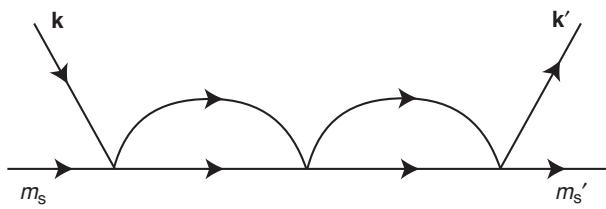
\includegraphics[width=0.6\textwidth]{figs/ch08/fig_8.11.jpg}
\caption*{图 8.11\quad 对标度给出线性修正的三阶近藤图（见习题 8.4）。}\label{fig:auto:8.11}
\end{figure}

最后一项
\begin{equation*}
H_{\mathrm{ch}} = -\frac{1}{2} \sum_{\mathbf{k},\mathbf{k}',\sigma} \big( B_{\mathbf{k}} V_{\mathbf{k}'d} \rho_{\mathbf{k}\sigma} \rho_{\mathbf{k}'-\sigma} + \mathrm{h.c.} \big),
\tag{8.129}
\end{equation*}
来源于式 (8.118) 的第三项，它使 d 杂质的占据数改变 2，因此对近藤问题同样不重要。相互作用中两个重要的项，是自旋交换过程和直接的杂质--电子散射项。

让我们把对应于杂质单占据的项分离出来。首先注意到，由于 $H_{\mathrm{ch}}$ 把 d 杂质上的两个电子都移走，它无法与希尔伯特空间中的单电子态相联系，我们舍去这一项。此外，在单电子子空间中 $\Psi_{d}^{\dagger} \Psi_{d} = 1$。因此，$H_{\mathrm{dir}}$ 是一个单电子项，$H_{0}'$ 与 $H_{0}''$ 也是。在这个子空间中，$H_{\mathrm{exch}}$ 是唯一重要的项。准确到 $V_{\mathbf{k}d}$ 的二阶，Anderson 模型给出具有反铁磁交换耦合的近藤模型。正是这一相互作用的反铁磁性质，导致了 d 杂质处向单态的凝聚。

\section*{习题}
\addcontentsline{toc}{section}{习题}

\textbf{习题 8.1}\quad (a) 大小固定的磁矩，其能量在磁场中是线性的。证明：这种磁矩的无相互作用集合的高温（居里）磁化率与 $T$ 成反比。

(b) 另一方面，可极化单态的能量在磁场中是二次的。证明：这种磁矩的无相互作用集合的磁化率在低温下趋于常数。

\textbf{习题 8.2}\quad 在杂质与导带电子之间存在铁磁自旋--自旋相互作用的情形下，重复 Yosida 的单电子变分计算，导出一个三重态束缚态。求解相应的三重态稳定性方程，并计算三重态的结合能。与单态相比，在相同的 $|J_{0}|$ 下哪一个能量更低？

\textbf{习题 8.3}\quad 求解各向异性标度方程（解析地或数值地），并验证它们满足图 8.10 所示的流图。

\textbf{习题 8.4}\quad 考虑图 8.11 所示的三阶近藤图。解释这幅图如何能给出一个线性于 $\delta D$ 的标度修正。假定 $\mathbf{q}$ 与 $\mathbf{q}'$ 相互独立。显式地计算标度系数。

\textbf{习题 8.5}\quad 利用由 Schrieffer--Wolff 变换导出的完整哈密顿量，即式 (8.124)，计算最低阶散射振幅：$T[(\mathbf{k}\sigma)+(d-\sigma) \to (\mathbf{k}'\sigma)+(d-\sigma)]$、$T[(\mathbf{k}\sigma)+(d\sigma) \to (\mathbf{k}'\sigma)+(d\sigma)]$ 与 $T[(\mathbf{k}\sigma)+(d-\sigma) \to (\mathbf{k}'-\sigma)+(d\sigma)]$，并与 8.2 节给出的结果比较。

\section*{参考文献}
\addcontentsline{toc}{section}{参考文献}

\begin{itemize}[leftmargin=2em,itemsep=0pt,parsep=0pt,label={}]
\item {[A1957]} A. A. Abrikosov, \emph{Physics} \textbf{2}, 5 (1965).
\item {[AL1991]} I. Affleck and A. W. W. Ludwig, \emph{Nucl. Phys. B} \textbf{352}, 849 (1991).
\item {[A1964]} P. W. Anderson, \emph{Phys. Rev.} \textbf{124}, 41 (1961).
\item {[AYH1970]} P. W. Anderson, G. Yuval, and D. R. Hamann, \emph{Phys. Rev. B} \textbf{1}, 4464 (1970).
\item {[A1978]} P. W. Anderson, \emph{Rev. Mod. Phys.} \textbf{50}, 191 (1978).
\item {[AFL1983]} N. Andrei, K. Furuya, and J. H. Lowenstein, \emph{Rev. Mod. Phys.} \textbf{55}, 331 (1983).
\item {[AZ1996]} V. Barzykin and I. Affleck, \emph{Phys. Rev. Lett.} \textbf{76}, 4959 (1996).
\item {[FN1994]} A. Furusaki and N. Nagaosa, \emph{Phys. Rev. Lett.} \textbf{72}, 892 (1994).
\item {[GL1954]} M. Gell-Mann and F. Low, \emph{Phys. Rev.} \textbf{111}, 582 (1954).
\item {[GZ1972]} G. Gr\"{u}ner and A. Zawadowski, \emph{Solid St. Comm.} \textbf{11}, 663 (1972).
\item {[H1969]} A. J. Heeger, in \emph{Solid State Physics}, eds. F. Seitz, D. Turnbull, and H. Ehrenreich (Academic Press, New York, 1969), p.~283.
\item {[H1993]} A. C. Hewson, \emph{The Kondo Problem to Heavy Fermions} (Cambridge University Press, New York, 1993).
\item {[K1956]} T. Kasuya, \emph{Prog. Theor. Phys.} \textbf{16}, 45 (1956).
\item {[K1964]} J. Kondo, \emph{Prog. Theor. Phys.} \textbf{32}, 37 (1964).
\item {[L1981]} C. Lacroix, \emph{J. Phys. F: Metal Phys.} \textbf{11}, 2389 (1981).
\item {[LT1992]} D. H. Lee and J. Toner, \emph{Phys. Rev. Lett.} \textbf{72}, 892 (1992).
\item {[N1974]} P. Nozi\`{e}res, \emph{J. Low Temp. Phys.} \textbf{17}, 31 (1974).
\item {[SCL1964]} M. Sarachik, E. Corenzwit, and L. D. Longinotti, \emph{Phys. Rev. A} \textbf{135}, 1041 (1964).
\item {[SW1966]} J. R. Schrieffer and P. A. Wolff, \emph{Phys. Rev.} \textbf{149}, 491 (1966).
\item {[SZ1974]} J. Solyom and A. Zawadowski, \emph{J. Phys. F: Metal Phys.} \textbf{4}, 80 (1974).
\item {[TW1983]} A. M. Tsvelick and P. B. Wiegmann, \emph{Adv. in Phys.} \textbf{32}, 453 (1983).
\item {[V1946]} S. Vousovskii, \emph{Zh. Eksp. Teor. Fiz.} \textbf{16}, 981 (1946).
\item {[W1975]} K. Wilson, \emph{Rev. Mod. Phys.} \textbf{47}, 773 (1975).
\item {[Y1966]} K. Yosida, \emph{Phys. Rev.} \textbf{147}, 223 (1966).
\item {[Z1951]} C. Zener, \emph{Phys. Rev.} \textbf{81}, 440 (1951).
\end{itemize}
